\documentclass[12pt]{article}
\usepackage{amsmath,amsfonts}
\usepackage{enumerate}
\usepackage{graphicx}
\usepackage{float}

\renewcommand{\baselinestretch}{1}
\topmargin 0in \headheight 0.0in \textheight 9in \textwidth 6.5in
\oddsidemargin 0.1in \evensidemargin 0.1in

\begin{document}

\section*{Data Generation}

The dataset consists of 2,000 simulated images, each with a \(16 \times 16\) grid of 256 pixels, split evenly into groups A and B. For images in group A, the central \(8 \times 8\) region is subject to a \(\beta\) effect, which was adjusted visually to be noticeable yet minimal. Figure~\ref{fig:image1} displays an image without the \(\beta\) effect, Figure~\ref{fig:image2} shows the effect at a strength of 1.5, and Figure~\ref{fig:image3} at a strength of 2, with the latter chosen for subsequent analyses.

The \(\beta\) matrix values are zero except in the central region, and the \texttt{group\_ind} vector classifies images into groups A (1) and B (0). Noise, \(\epsilon_i\), is added to each image, derived from a multivariate normal distribution with zero mean and a covariance structure based on an exponential correlation function with rate 1.

Question about how to generate exponential correlation matrix: for any two pixels, \(\text{dist}(i, j) = \sqrt{(x_1 - x_2)^2 + (y_1 - y_2)^2}\). I found two ways to calculate the exponential correlation matrix online:
\begin{itemize}
    \item \(\text{cor}(i, j) = \exp(-\alpha \times \text{dist}(i, j))\), \(\alpha\) is called rate;
    \item \(\text{cor}(i, j) = \rho^{\text{dist}(i, j)}, \ \rho < 1\)
\end{itemize}
I think we are aiming at the first one?

% To adapt the data for the input specifications of the \texttt{myresf\_vc} function, the dataset was transformed into a long format. In this format, the columns \texttt{x} and \texttt{y} denote the coordinates, while \texttt{pixel\_value} corresponds to the simulated $y$ values.

\begin{figure}[H]
    \centering
    % First Row
    \begin{minipage}{0.45\textwidth}
        \centering
        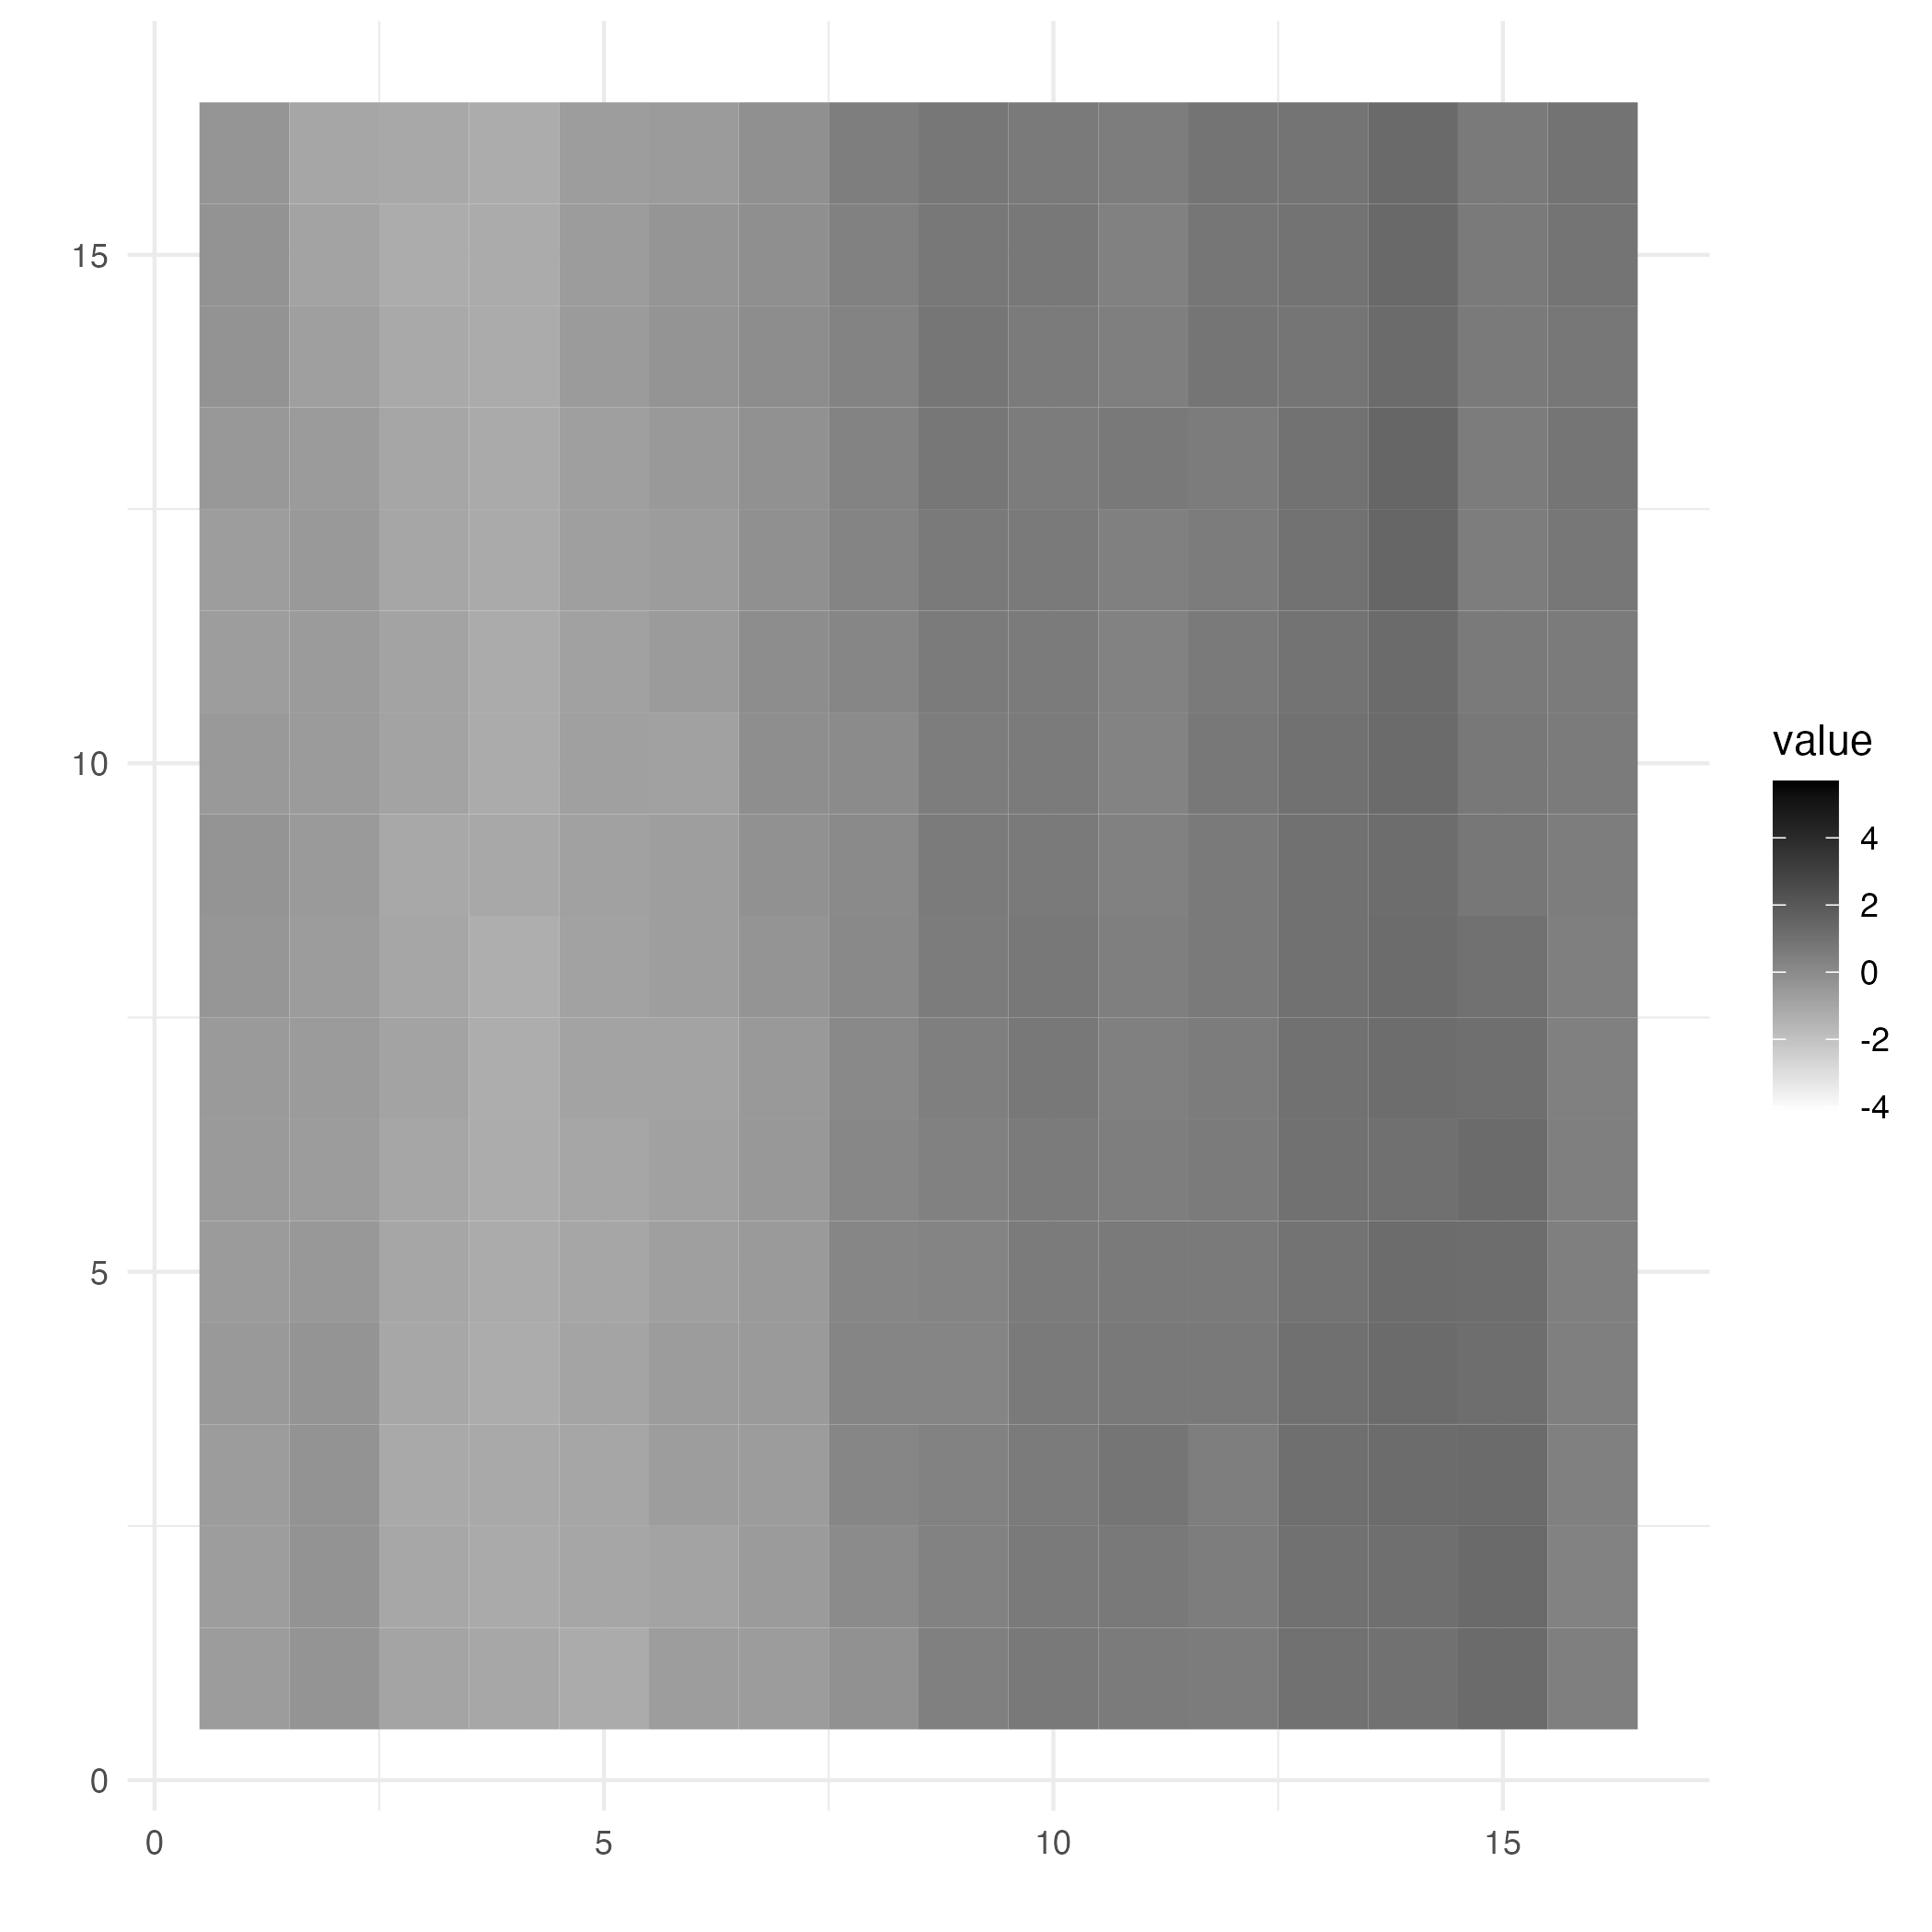
\includegraphics[width=0.9\textwidth]{../Figures/image_ex2c.png}
        \caption{Example image without \(\beta\) effect}
        \label{fig:image1}
    \end{minipage}\hfill
    \begin{minipage}{0.45\textwidth}
        \centering
        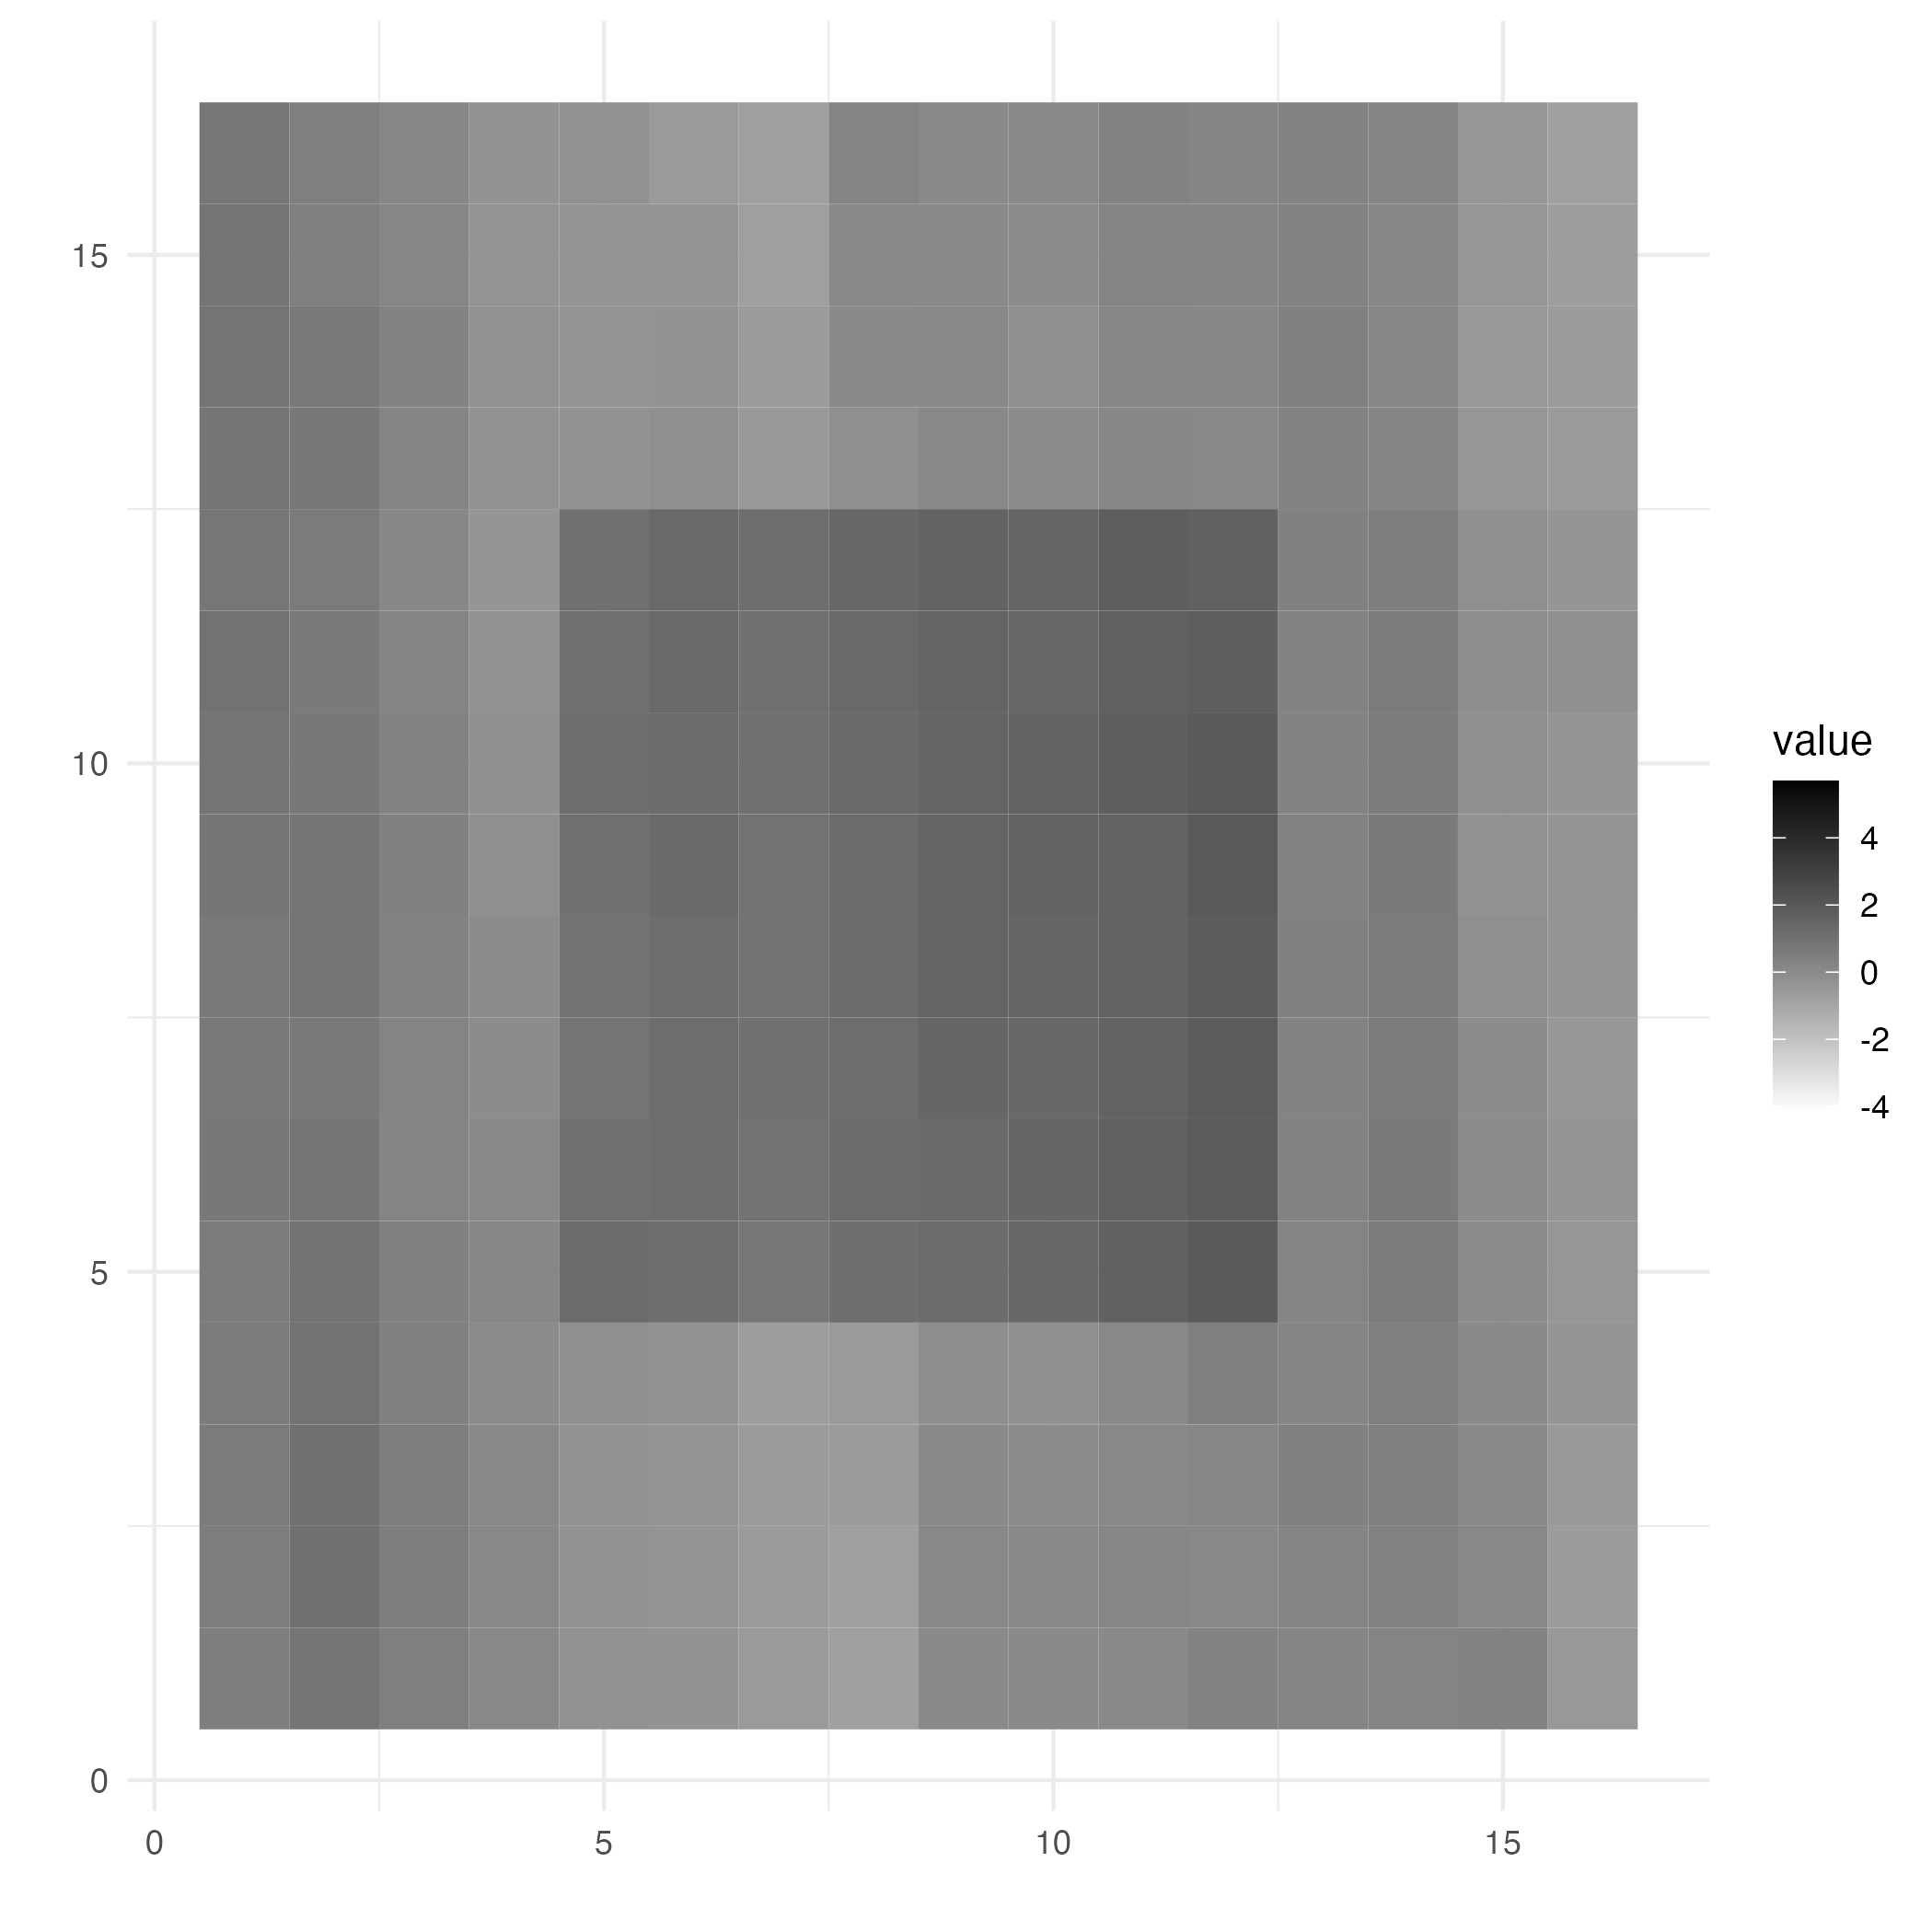
\includegraphics[width=0.9\textwidth]{../Figures/image_ex1_5.png}
        \caption{Example image with \(\beta = 1.5\)}
        \label{fig:image2}
    \end{minipage}

    % Second Row
    \begin{minipage}{0.45\textwidth}
        \centering
        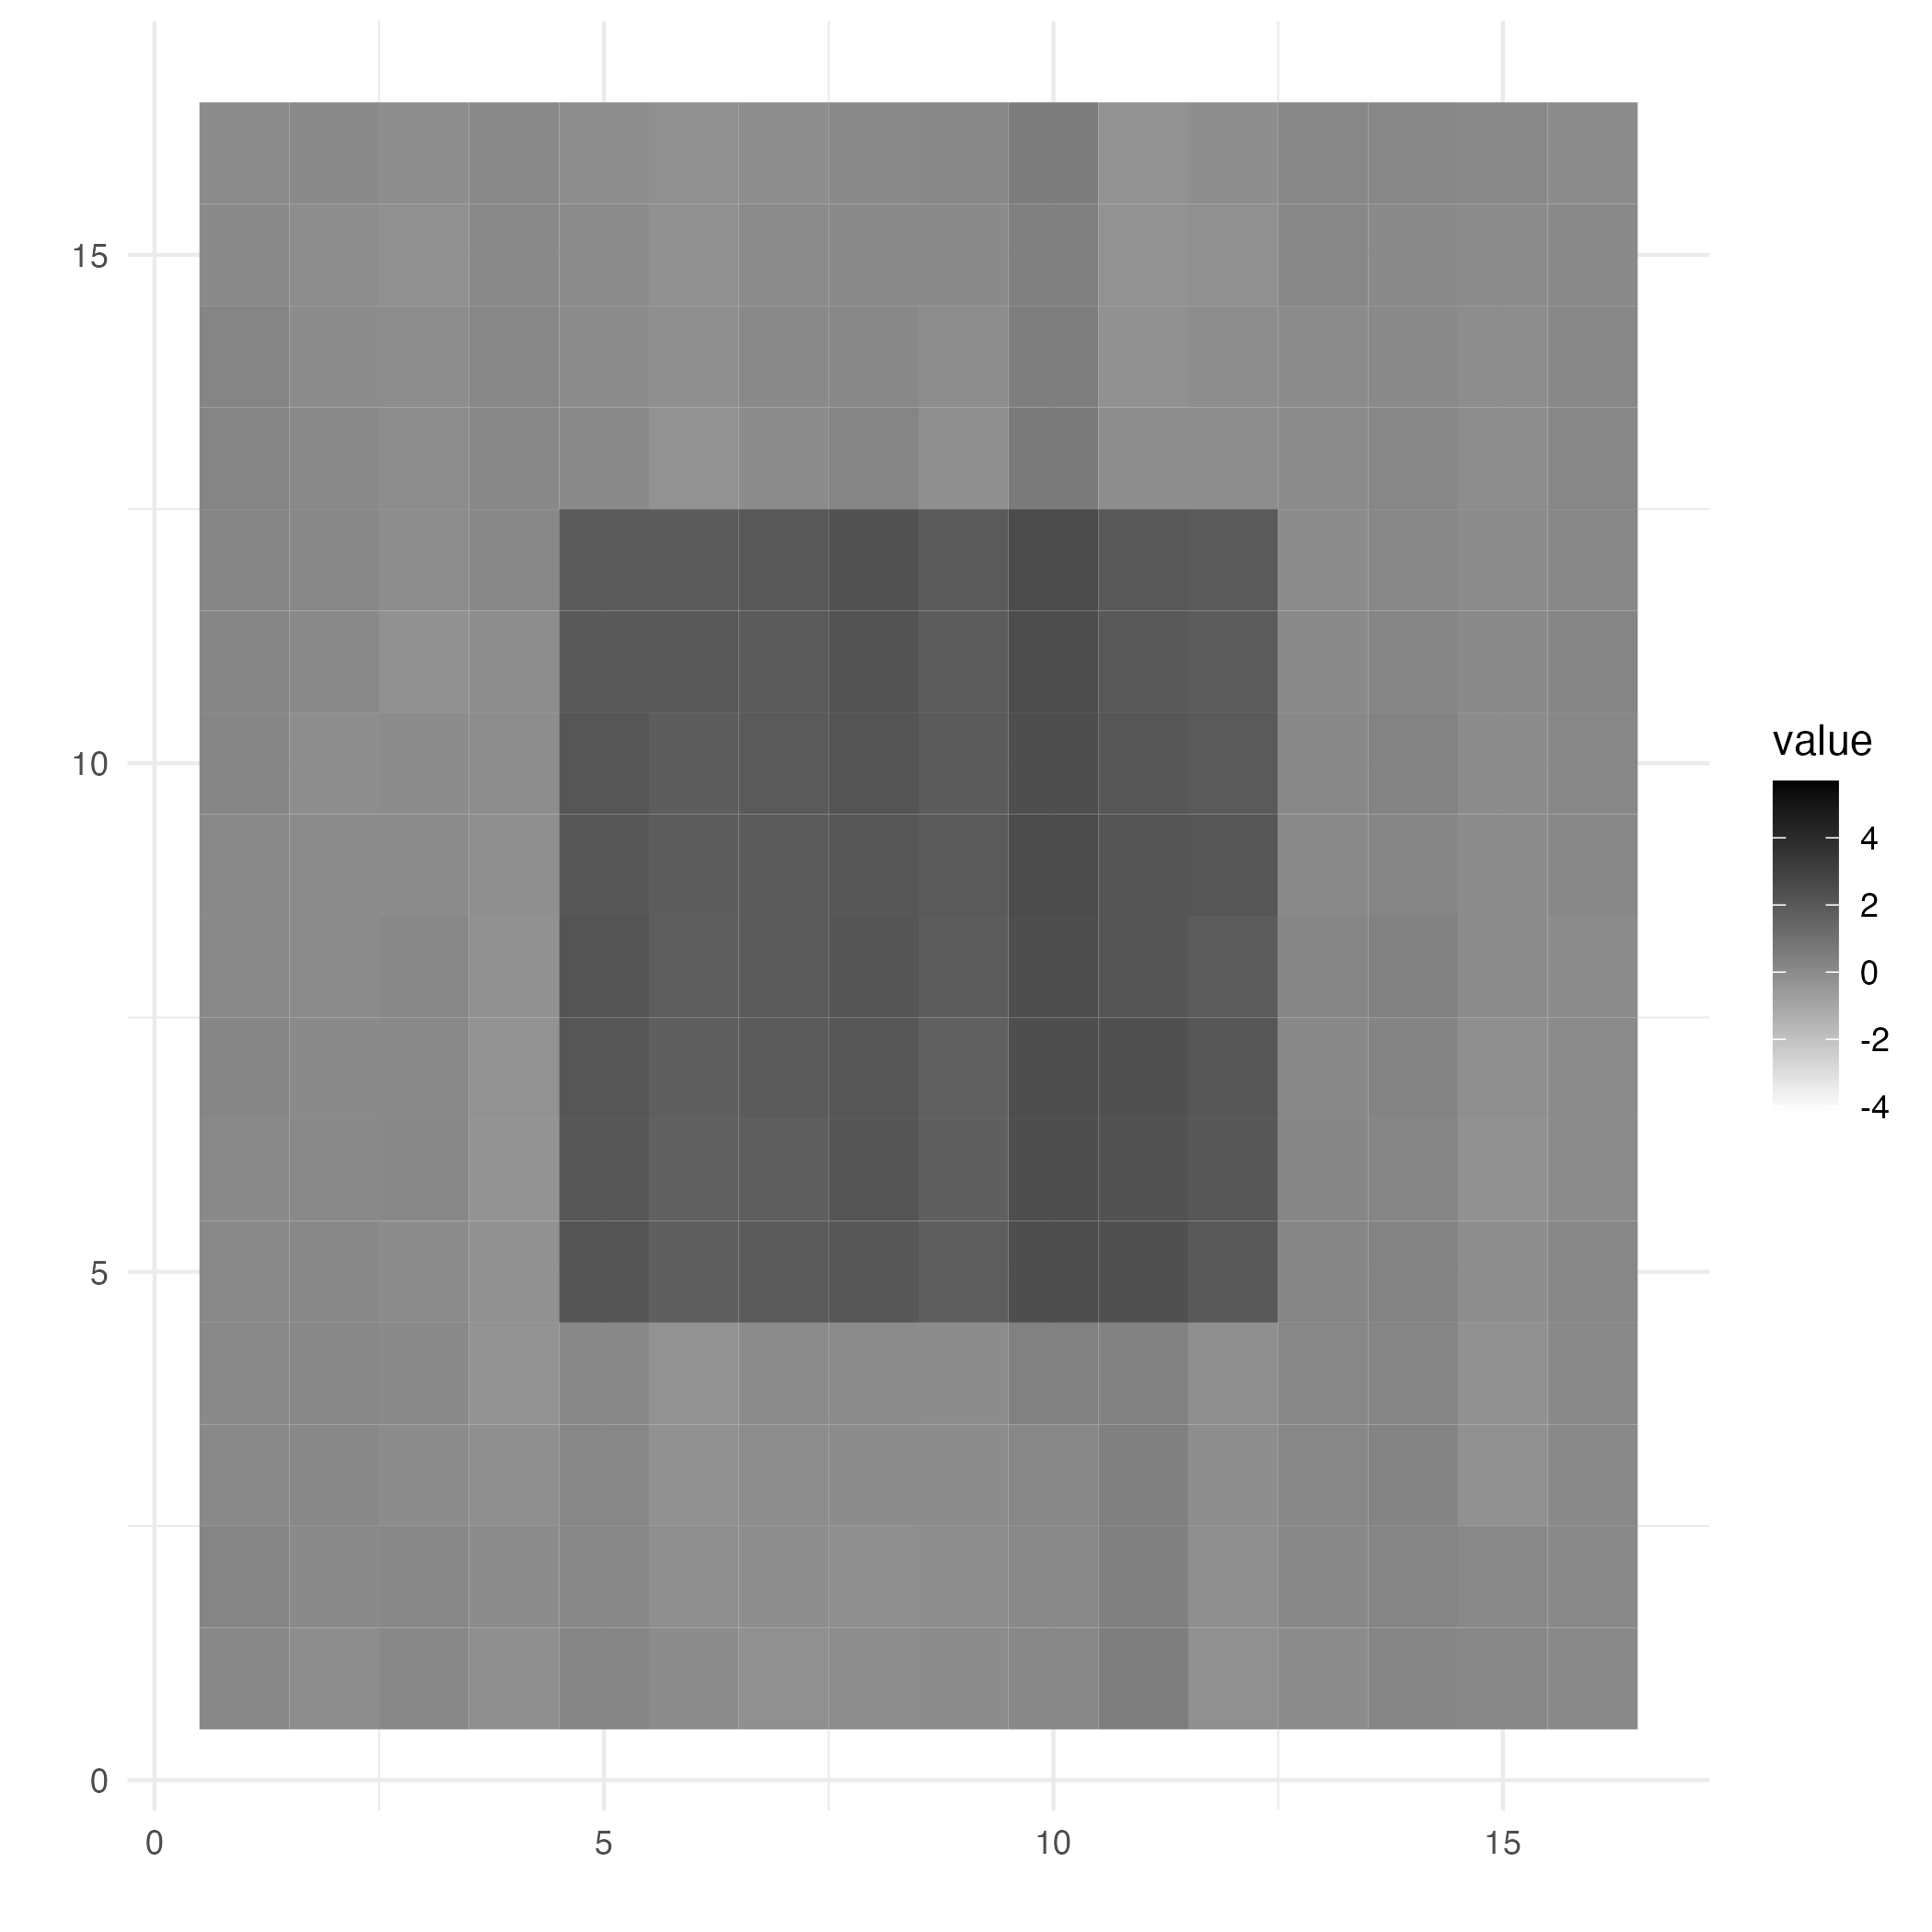
\includegraphics[width=0.9\textwidth]{../Figures/image_ex2.png}
        \caption{Example image with \(\beta = 2\)}
        \label{fig:image3}
    \end{minipage}\hfill
    \begin{minipage}{0.45\textwidth}
        % left blank
    \end{minipage}
\end{figure}

\section*{VBM}

In the VBM analysis, a Generalized Linear Model (GLM) was applied pixel-wise to assess group effects on pixel intensities across 100 iterations. For each iteration, the model generated effect size estimates and p-values for each pixel. These p-values were then corrected for multiple comparisons using the Bonferroni method. Figure \ref{fig:vbm_pvals} depicts the frequency of significant p-values in across pixels, with pixels showing significant \(\beta\) in all 100 iterations appearing in black, and those never showing significance in white.

\begin{figure}[H]
    \centering
    % First figure
    \begin{minipage}[b]{0.45\textwidth}
        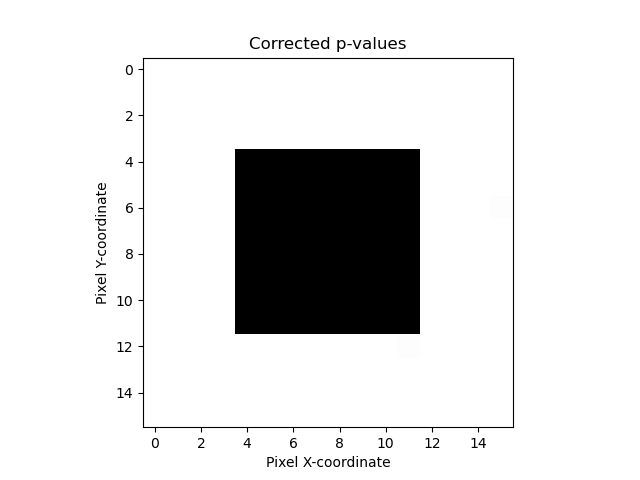
\includegraphics[width=\textwidth]{/Users/siyangren/Documents/ra-cida/ESFGSP_Paper/Figures/vbm_pvals.png}
        \caption{\% of significant p-values across pixels in VBM analysis}
    \end{minipage}
    \hfill % This command adds a space between the two figures
    % Second figure
    \begin{minipage}[b]{0.45\textwidth}
        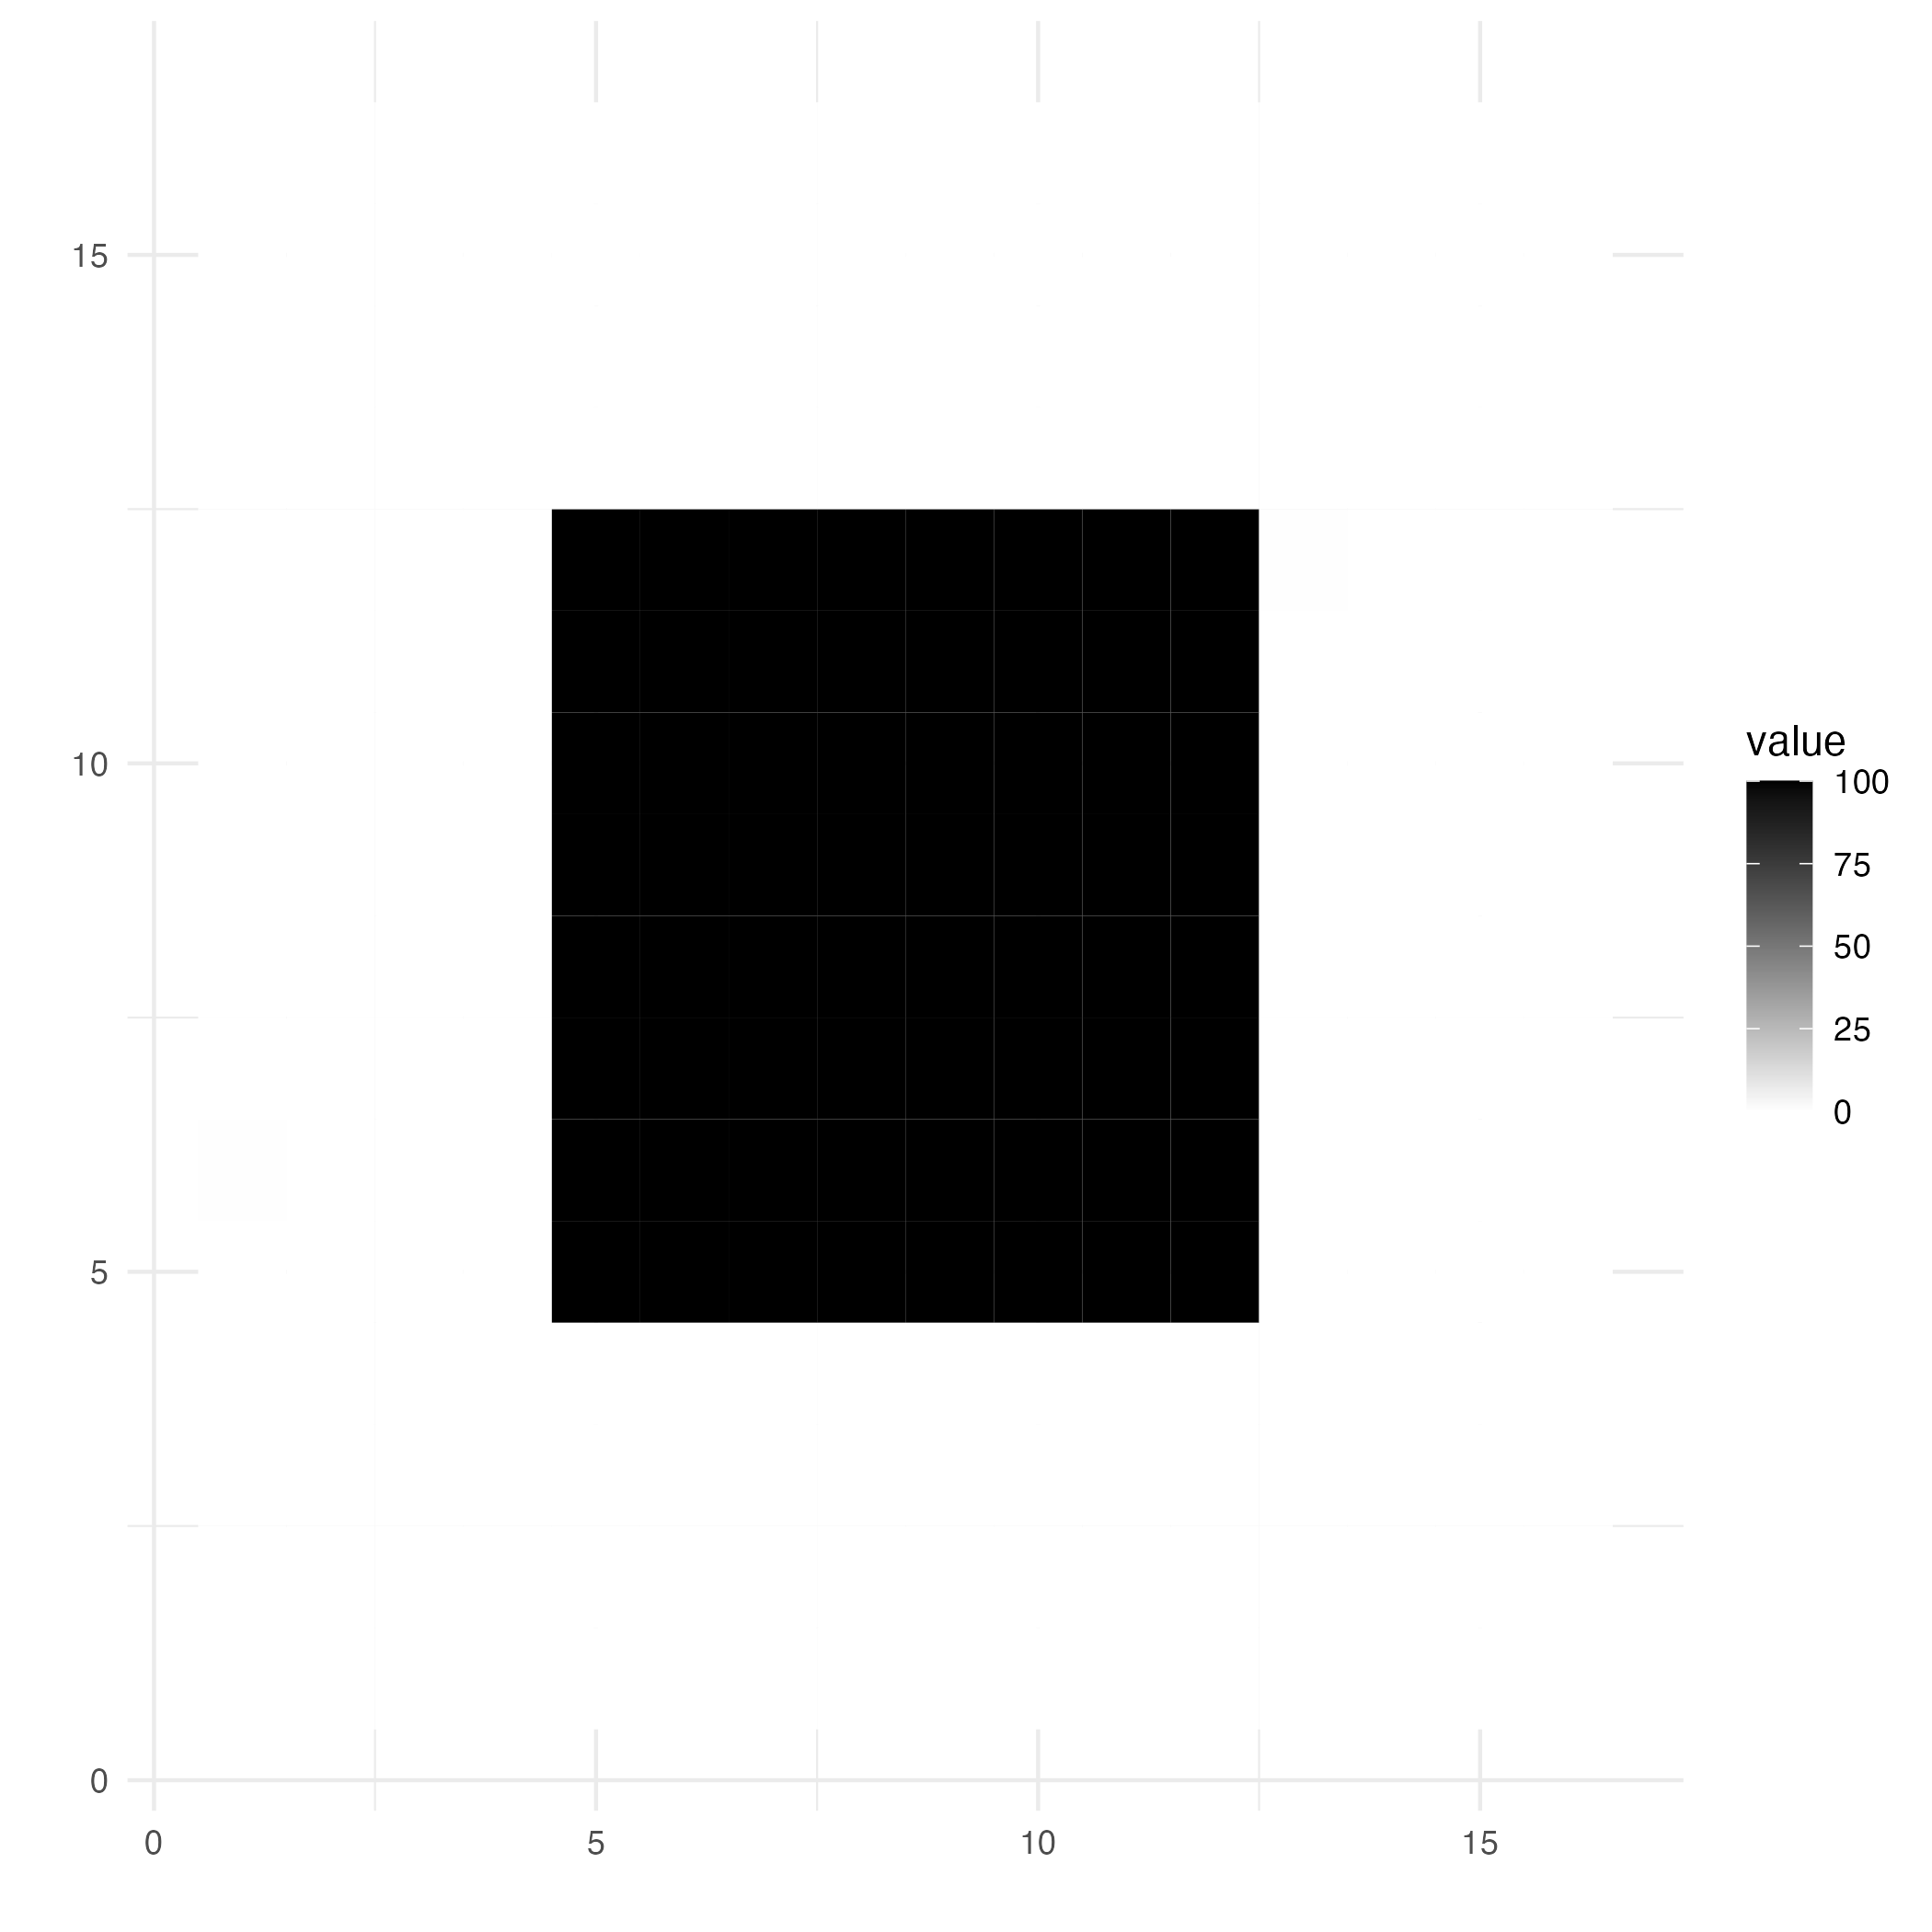
\includegraphics[width=\textwidth]{/Users/siyangren/Documents/ra-cida/ESFGSP_Paper/Figures/vbm_pvals_corr.png}
        \caption{\% of significant p-values after correction across pixels in VBM analysis}
    \end{minipage}
\end{figure}


\section*{spVBM}

The spVBM model is:
\[
    \begin{aligned}
         & y_s^i=\sum_{k=1}^K x_{s, k}^i \beta_{s, k}^{S V C}+\mathbf{Z}^{\mathbf{i}} \mathbf{b}^{\mathbf{i}}+\varepsilon_s^i                                                                                                                      \\
         & \beta_{s, k}^{S V C}=\beta_k+[\mathbf{E} \Gamma]_{s, k}                                                                                                                                                                                 \\
         & \mathbf{b}^{\mathbf{i}} \sim \mathcal{N}(\mathbf{0}, G), \quad \varepsilon_i \sim \mathcal{N}\left(0, \sigma^2\right), \quad \Gamma_{, k} \sim \mathcal{N}\left(\mathbf{0}, \sigma_k^2 \boldsymbol{\Lambda}\left(\alpha_k\right)\right)
    \end{aligned}
\]
\(y_s^i\) denote the spatial outcome for subject \(i\) voxel \(s\). \(\mathbf{Z}\) denote non-spatial subject-level covariates for non-spatial random effects.

In our simulated data, this could be simplified to \(y_s^i = x_s^i \beta_s^{SVC} + (?) \). My question is, which term captures the exponential correlation structure in the model? \(G\) or \(\Gamma\)?

\begin{figure}[H]
    \centering
    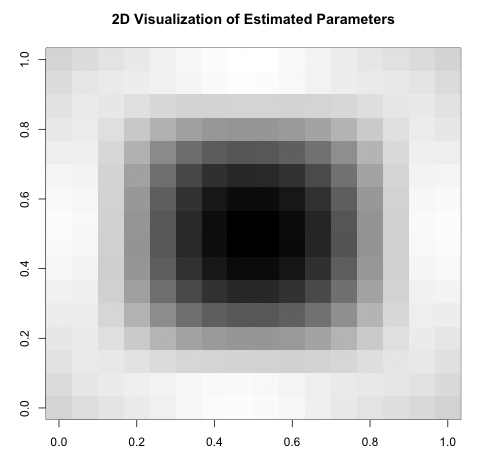
\includegraphics[width=0.5\textwidth]{/Users/siyangren/Documents/ra-cida/ESFGSP_Paper/Figures/spvbm_coefs_april_3.png}
    \caption{Estimated coefficients}
    \label{fig:my_label}
\end{figure}

\section*{LASSO}

A LASSO model was employed to predict group assignments using pixel values from images. In each iteration, 80\% of the data was used for training and the remaining 20\% for testing. The optimal \(\lambda\) parameters, \texttt{lambda\_min} and \texttt{lambda\_1se}, were determined via cross-validation within the training group. The model's performance was assessed on the test group using accuracy and AUC metrics.

Initially, including all pixel values in the model led to perfect separation, indicating potential overfitting. To address this, the model construction began by incrementally adding one pixel from the image's edge and one from the center, evaluating if these additions achieved perfect accuracy. After integrating three pairs of pixels, totaling six pixels, the model achieved perfect separation.

Additionally, a permutation test was conducted to estimate p-values.

\begin{figure}[H]
    \centering
    % First figure
    \begin{minipage}[b]{0.45\textwidth}
        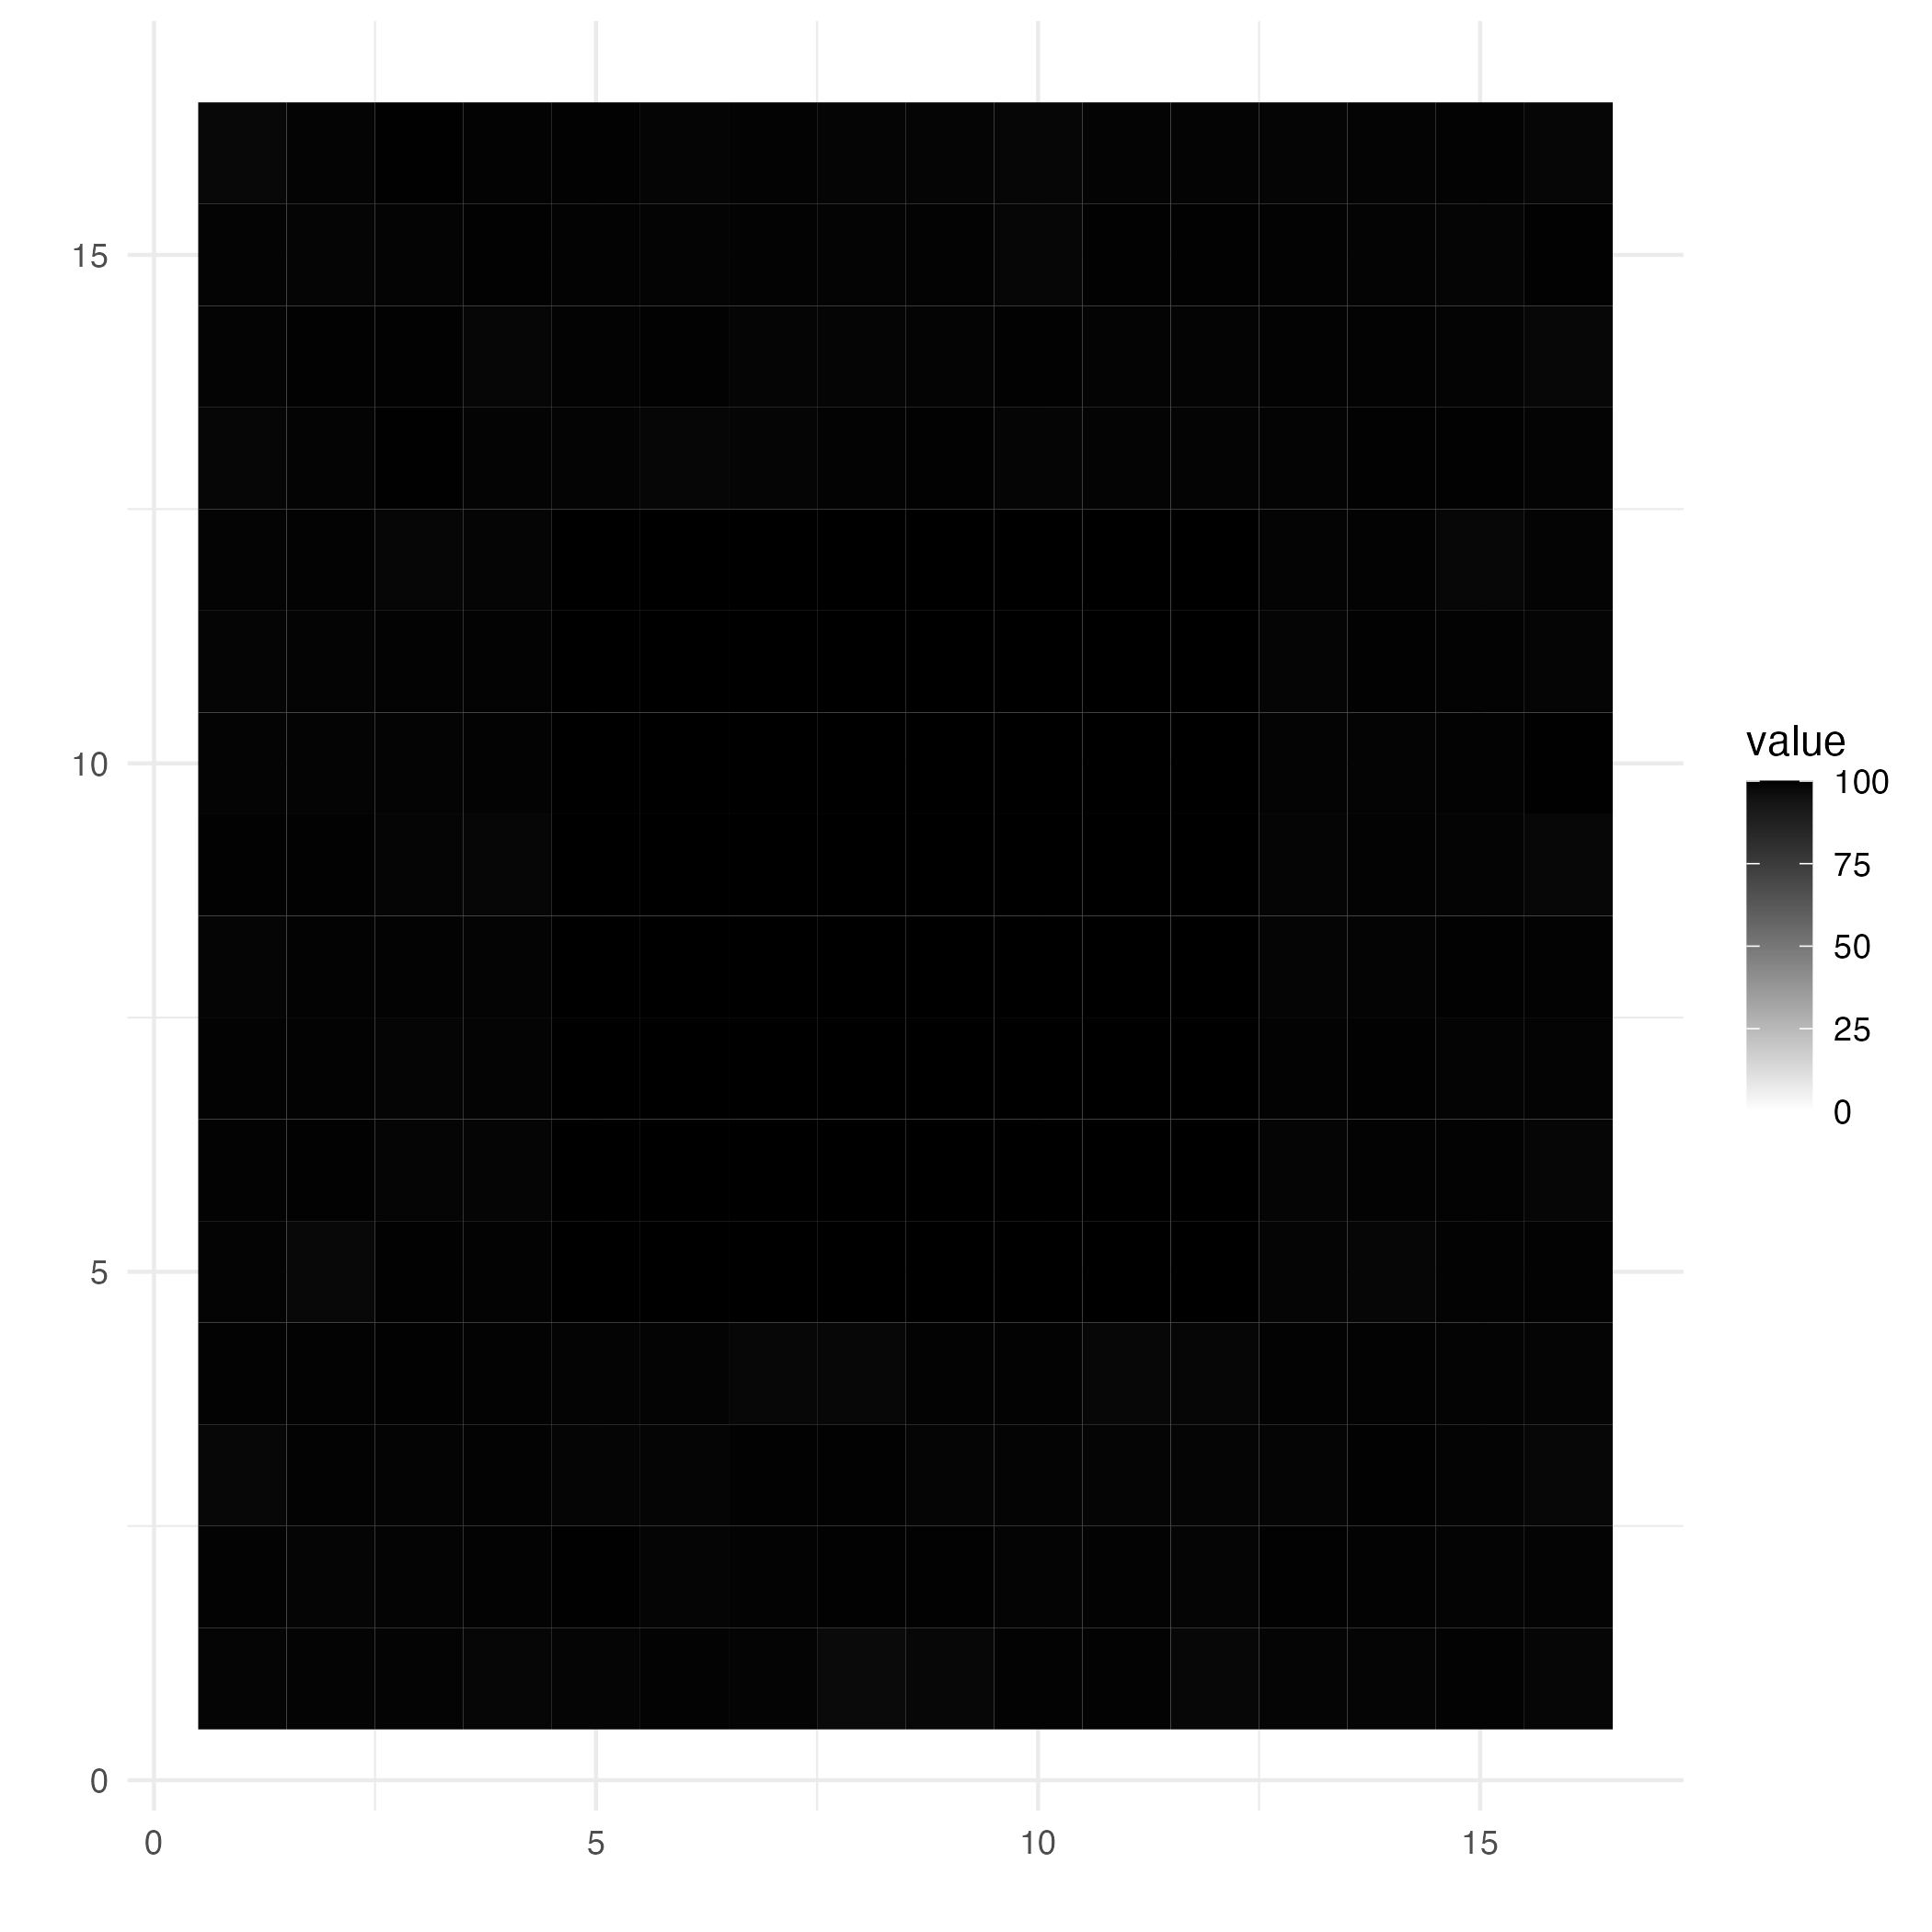
\includegraphics[width=\textwidth]{../Figures/lasso_pvals.png}
        \caption{\% of significant p-values across pixels in LASSO}
    \end{minipage}
    \hfill % This command adds a space between the two figures
    % Second figure
    \begin{minipage}[b]{0.45\textwidth}
        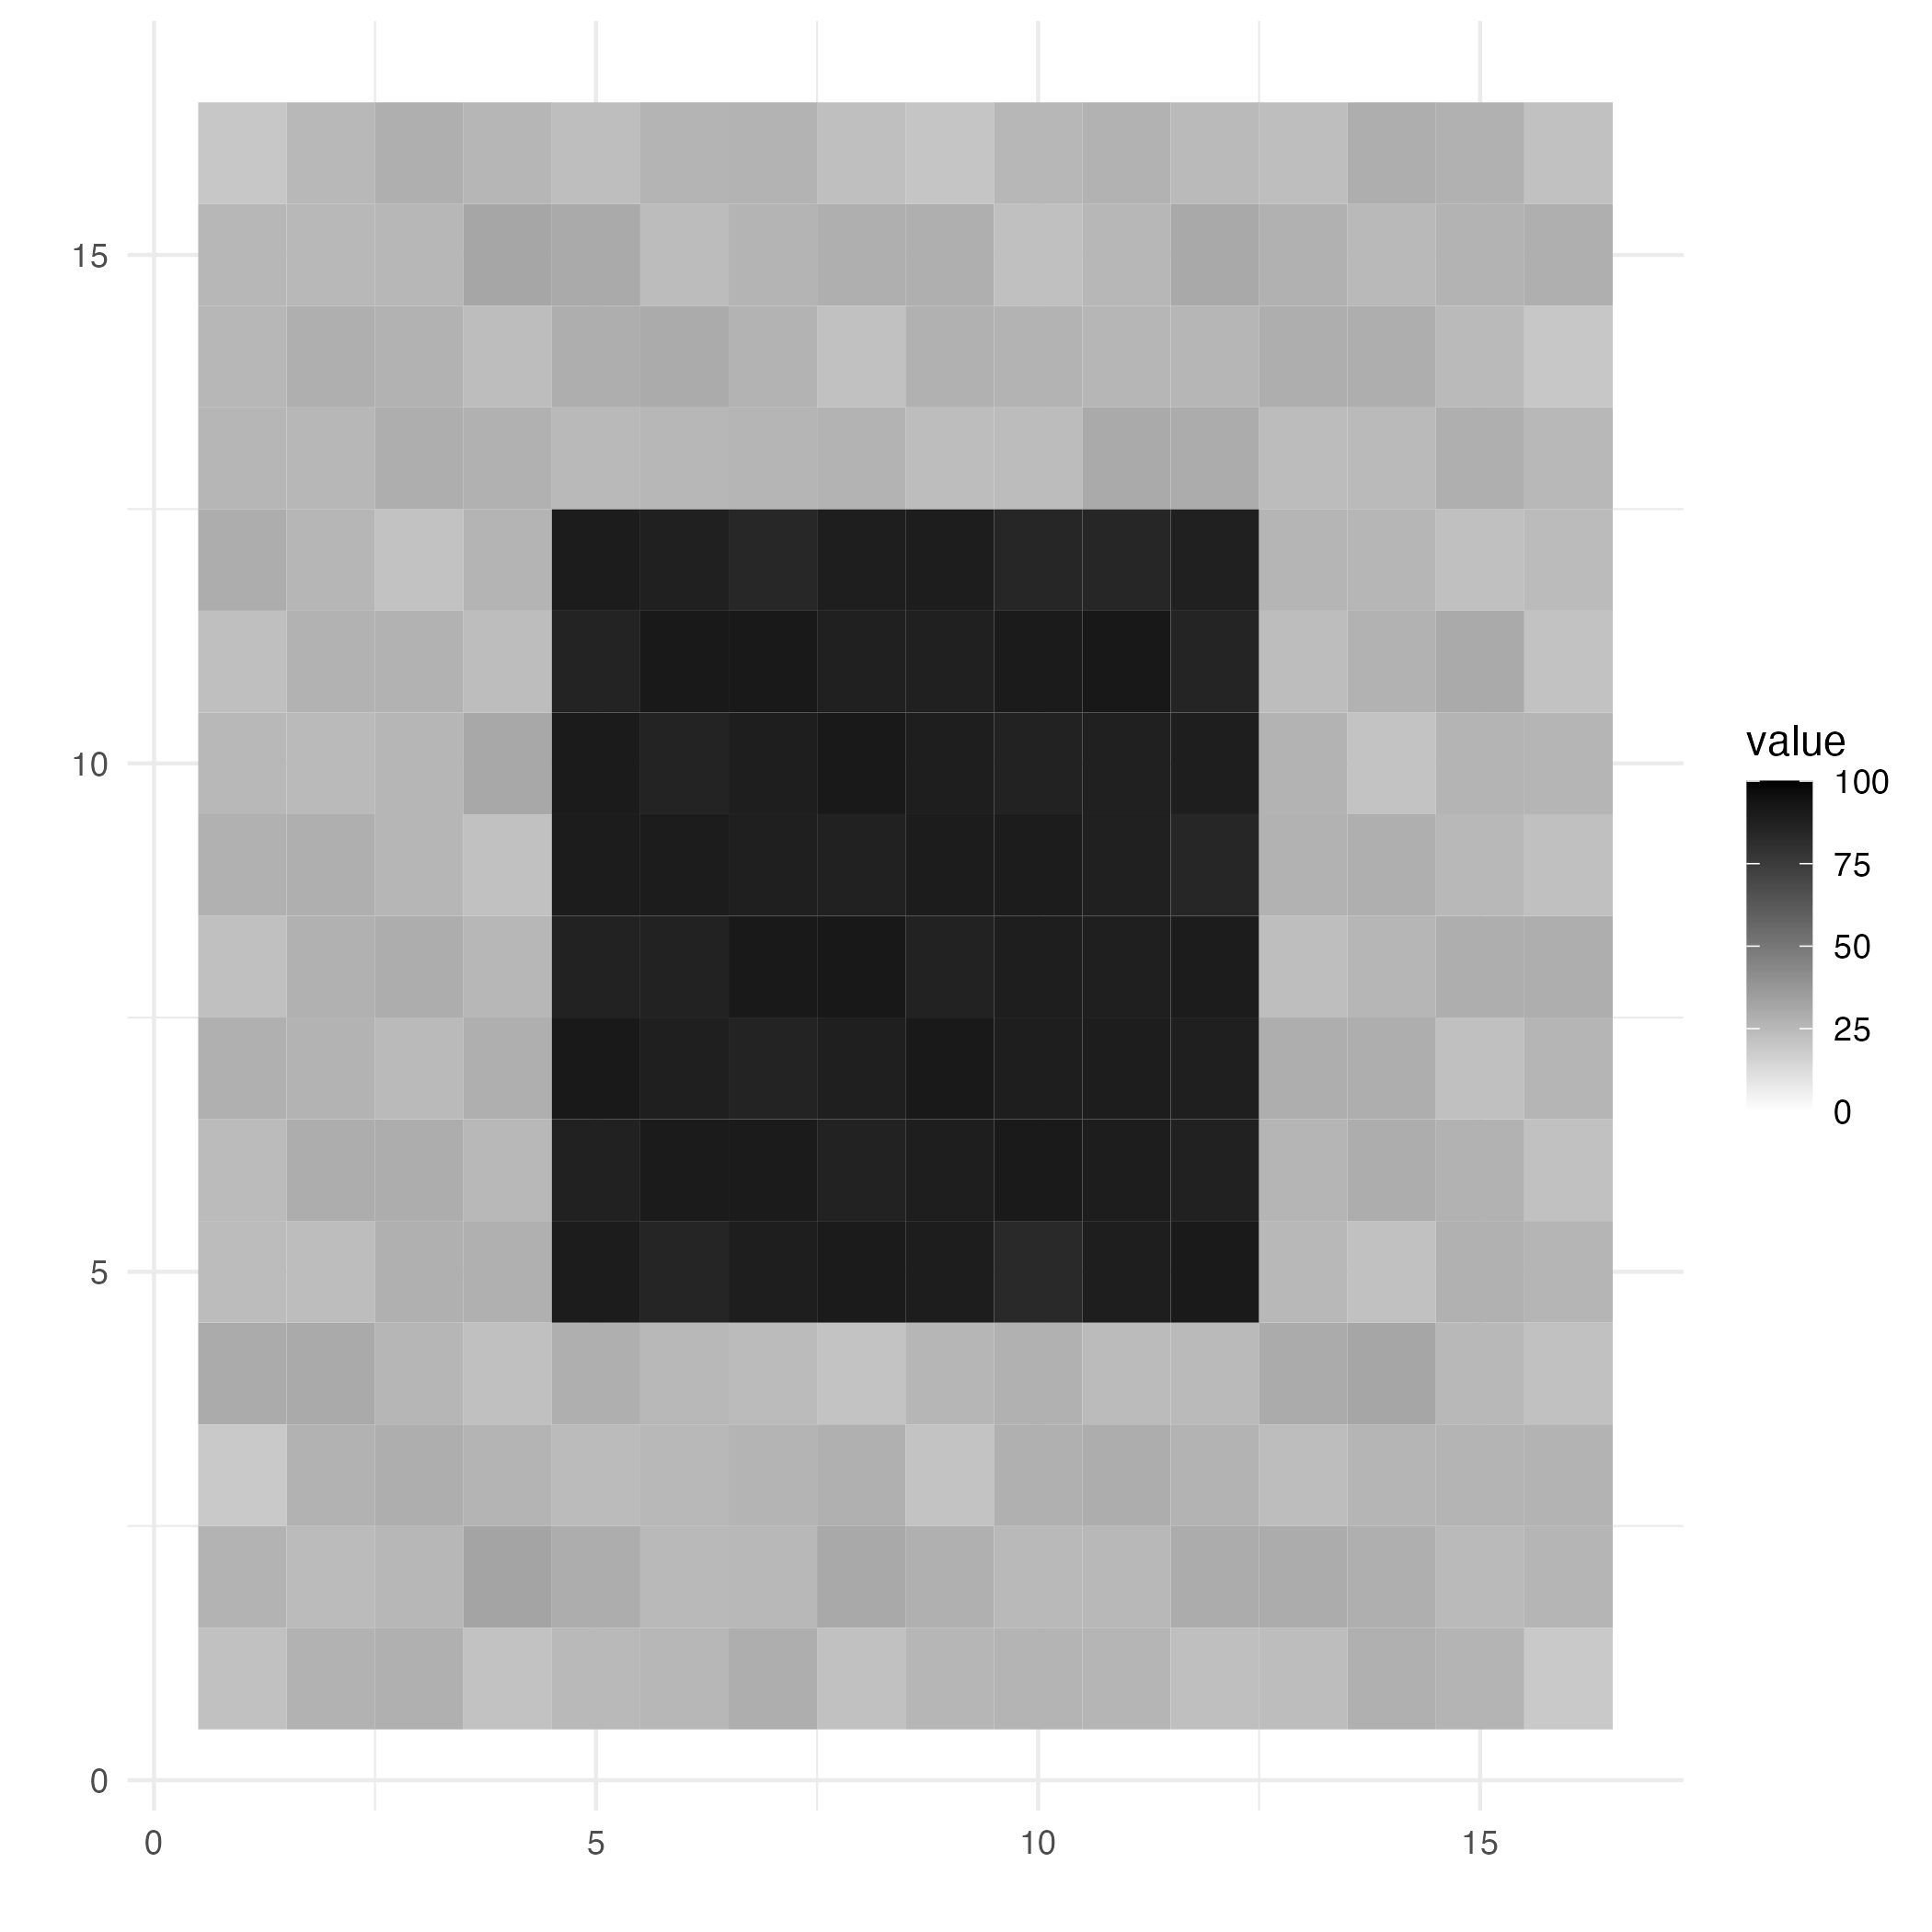
\includegraphics[width=\textwidth]{../Figures/lasso_pvals_corr.png}
        \caption{\% of significant p-values after correction across pixels in LASSO}
    \end{minipage}
\end{figure}


\section*{Frequency}

An empirical correlation matrix was computed from the \(2000 \times 256\) pixel matrix, followed by the extraction of eigenvectors and eigenvalues. The dataset X was then transformed using the eigenvectors corresponding to positive eigenvalues. A Lasso regression model was fitted on the transformed data to predict \texttt{group\_ind}. The significance of the model coefficients was assessed using p-values obtained from 1000 permutation tests.

\end{document}
